\documentclass{beamer}
\mode<presentation> {
%\usetheme{Madrid}
%\usetheme{default}
\usepackage{color}
\definecolor{bottomcolour}{rgb}{0.21,0.11,0.21}
\definecolor{middlecolour}{rgb}{0.21,0.11,0.21}
\setbeamercolor{structure}{fg=white}
\setbeamertemplate{frametitle}[default]%[center]
\setbeamercolor{normal text}{bg=black, fg=white}
\setbeamertemplate{background canvas}[vertical shading]
[bottom=bottomcolour, middle=middlecolour, top=black]
\setbeamertemplate{items}[circle]
\setbeamertemplate{navigation symbols}{} %no nav symbols
\setbeamercolor{block title}{use=structure,fg=white,bg=structure.fg!50!red!50!blue!100!green}
\setbeamercolor{block body}{parent=normal text,use=block title,bg=block title.bg!5!white!10!bg,fg=white}
\setbeamertemplate{navigation symbols}{}
}
\usepackage{graphicx} 
\usepackage{booktabs} 
\usepackage[utf8]{inputenc}  
\usepackage[T1]{fontenc}  
\usepackage{geometry}     
\usepackage[francais]{babel} 
\usepackage{eurosym}
\usepackage{verbatim}
\usepackage{ragged2e}
\justifying
%%%%%%%%%%%%%%%%%%%%%%%%%%%%%%%%%%%%%%%%%%%%%%%%%%%%%%%%%%%%%%%%
%% ccBeamer 0.1, 2007-07-02                                   %%
%% Written by Sebastian Pipping <webmaster@hartwork.org>      %%
%% ---------------------------------------------------------- %%
%% Licensed under Creative Commons Attribution-ShareAlike 3.0 %%
%% http://creativecommons.org/licenses/by-sa/3.0/             %%
%%%%%%%%%%%%%%%%%%%%%%%%%%%%%%%%%%%%%%%%%%%%%%%%%%%%%%%%%%%%%%%%


%% Images
\newcommand{\CcImageBy}[1]{%
	
\includegraphics[scale=#1]{creative_commons/cc_by_30.pdf}%
}
\newcommand{\CcImageCc}[1]{%
	
\includegraphics[scale=#1]{creative_commons/cc_cc_30.pdf}%
}
\newcommand{\CcImageDevNations}[1]{%
	
\includegraphics[scale=#1]{creative_commons/cc_dev_nations_30.pdf}%
}
\newcommand{\CcImageNc}[1]{%
	
\includegraphics[scale=#1]{creative_commons/cc_nc_30.pdf}%
}
\newcommand{\CcImageNd}[1]{%
	
\includegraphics[scale=#1]{creative_commons/cc_nd_30.pdf}%
}
\newcommand{\CcImagePd}[1]{%
	
\includegraphics[scale=#1]{creative_commons/cc_pd_30.pdf}%
}
\newcommand{\CcImageSa}[1]{%
	
\includegraphics[scale=#1]{creative_commons/cc_sa_30.pdf}%
}
\newcommand{\CcImageSampling}[1]{%
	
\includegraphics[scale=#1]{creative_commons/cc_sampling_30.pdf}%
}
\newcommand{\CcImageSamplingPlus}[1]{%
	
\includegraphics[scale=#1]{creative_commons/cc_sampling_plus_30.pdf}%
}


%% Groups
\newcommand{\CcGroupBy}[1]{% zoom
	\CcImageBy{#1}%
}
\newcommand{\CcGroupByNc}[2]{% zoom, gap
	\CcImageBy{#1}\hspace*{#2}\CcImageNc{#1}%
}
\newcommand{\CcGroupByNcNd}[2]{% zoom, gap
	\CcImageBy{#1}\hspace*{#2}\CcImageNc{#1}\hspace*{#2}\CcImageNd{#1}%
}
\newcommand{\CcGroupByNcSa}[2]{% zoom, gap
	\CcImageBy{#1}\hspace*{#2}\CcImageNc{#1}\hspace*{#2}\CcImageSa{#1}%
}
\newcommand{\CcGroupByNd}[2]{% zoom, gap
	\CcImageBy{#1}\hspace*{#2}\CcImageNd{#1}%
}
\newcommand{\CcGroupBySa}[2]{% zoom, gap
	\CcImageBy{#1}\hspace*{#2}\CcImageSa{#1}%
}
\newcommand{\CcGroupDevNations}[1]{% zoom
	\CcImageDevNations{#1}%
}
\newcommand{\CcGroupNcSampling}[2]{% zoom, gap
	\CcImageNc{#1}\hspace*{#2}\CcImageSampling{#1}%
}
\newcommand{\CcGroupPd}[1]{% zoom
	\CcImagePd{#1}%
}
\newcommand{\CcGroupSampling}[1]{% zoom
	\CcImageSampling{#1}%
}
\newcommand{\CcGroupSamplingPlus}[1]{% zoom
	\CcImageSamplingPlus{#1}%
}


%% Text
\newcommand{\CcLongnameBy}{Attribution}
\newcommand{\CcLongnameByNc}{Attribution-NonCommercial}
\newcommand{\CcLongnameByNcNd}{Attribution-NoDerivs}
\newcommand{\CcLongnameByNcSa}{Attribution-NonCommercial-ShareAlike}
\newcommand{\CcLongnameByNd}{Attribution-NoDerivs}
\newcommand{\CcLongnameBySa}{Attribution-ShareAlike}

\newcommand{\CcNote}[1]{% longname
	This work is licensed under the \textit{Creative Commons #1 3.0 License}.%
}

\title[Tor et le Tor Browser Bundle]{Ubuntu Party \\ Le réseau Tor} 
\author{Genma - Café vie privée}
\begin{document}
%% Titlepage
\begin{frame}
	\titlepage
	\vfill
	\begin{center}
		
\includegraphics[scale=0.2]{./images/logo_tor.jpg}
		\\		
		\CcGroupByNcSa{0.83}{0.95ex}\\[2.5ex]
		{\tiny\CcNote{\CcLongnameByNcSa}}
		\vspace*{-2.5ex}
	\end{center}
\end{frame}

\begin{frame}
\frametitle{
\includegraphics[scale=0.4]{./images/Genma.jpg} \ \ \  A propos de moi  }
\begin{columns}[c] 

\column{.55\textwidth} 
\textbf{Où me trouver sur Internet?}
\begin{itemize}
\item Le Blog de Genma : http://genma.free.fr
\item Twitter : http://twitter.com/genma
\end{itemize}
\textbf{Mes centres d'intérêts?}
\\ Plein de choses dont:
\begin{itemize}
\item Organiser des Cafés vie privée
\end{itemize}
\column{.5\textwidth} 
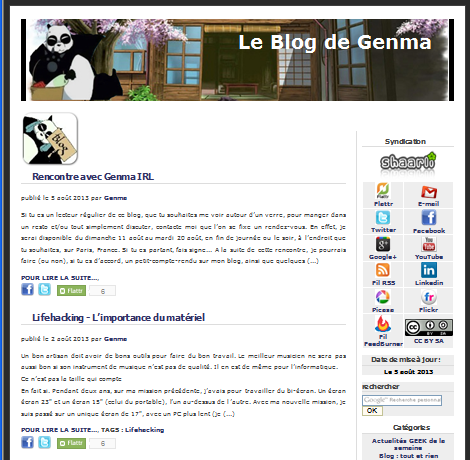
\includegraphics[width=5cm,height=5cm]{./images/blog.png} 
\end{columns}
\end{frame}

%----------------------------------------------------------------------------------------
\begin{frame}
\frametitle{Remerciements}
Je remercie l'association NosOignons.net, qui propose des nœuds de sortie Tor financés par la communauté.
\url{https://nos-oignons.net}
\\~\\

\includegraphics[scale=0.4]{./images/NosOignons.jpg}
\end{frame}
%----------------------------------------------------------------------------------------
\begin{frame}
\begin{center}
\Huge{Introduction}
\\~\\ 
\includegraphics[scale=0.4]{./images/logo_tor.jpg}
\end{center}
\end{frame}
%----------------------------------------------------------------------------------------
\begin{frame}
\frametitle{Présentation du réseau TOR}
Tor est un logiciel libre,
\begin{itemize}
\item grâce auquel existe le réseau d'anonymisation Tor
\item  soutenu par l'organisation The Tor Project.
\end{itemize}
$\Rightarrow$ Techniquement, Tor nous permet de se connecter à des machines sur Internet via des relais. 
\\$\Rightarrow$ Et cela de façon à ce qu'elles ne puissent pas identifier notre connexion (et donc de nous localiser).
\end{frame}
%----------------------------------------------------------------------------------------
\begin{frame}
\begin{center}
\Huge{A quoi sert TOR?}
\\~\\ 
\includegraphics[scale=0.4]{./images/logo_tor.jpg}
\end{center}
\end{frame}
%----------------------------------------------------------------------------------------
\begin{frame}
\frametitle{A quoi sert TOR?}
Concrêtement, ça sert pour :
\begin{itemize}
\item  échapper au fichage publicitaire,
\item  publier des informations sous un pseudonyme,
\item  accéder à des informations en laissant moins de traces,
\item  déjouer des dispositifs de filtrage (dans sa fac, en Chine ou en Iran…),
\item  communiquer en déjouant des dispositifs de surveillances,
\item  tester son pare-feu,
\item  … et sûrement encore d'autres choses.
\end{itemize}
$\Rightarrow$ Tor dispose également d'un système de « services cachés » qui permet de fournir un service en cachant l'emplacement du serveur.
\end{frame}
%----------------------------------------------------------------------------------------
\begin{frame}
\frametitle{A quoi sert TOR?}
Tor est un réseau d'anonymisation, donc par définition, c'est difficile de faire un compte
précis.Tor ne fait rien pour cacher que nous utilisons Tor. Donc quand en utilisant
Tor, nous nous mettons au milieu de la foule des gens qui utilisent Tor. Plus
cette foule est grande, meilleur est l'anonymat.
\end{frame}
%----------------------------------------------------------------------------------------
\begin{frame}
\begin{center}
\Huge{Comment fonctionne Tor ? }
\\~\\ 
\includegraphics[scale=0.4]{./images/logo_tor.jpg}
\end{center}
\end{frame}
%----------------------------------------------------------------------------------------
\begin{frame}
\frametitle{Comment fonctionne Tor ?}
\begin{center}
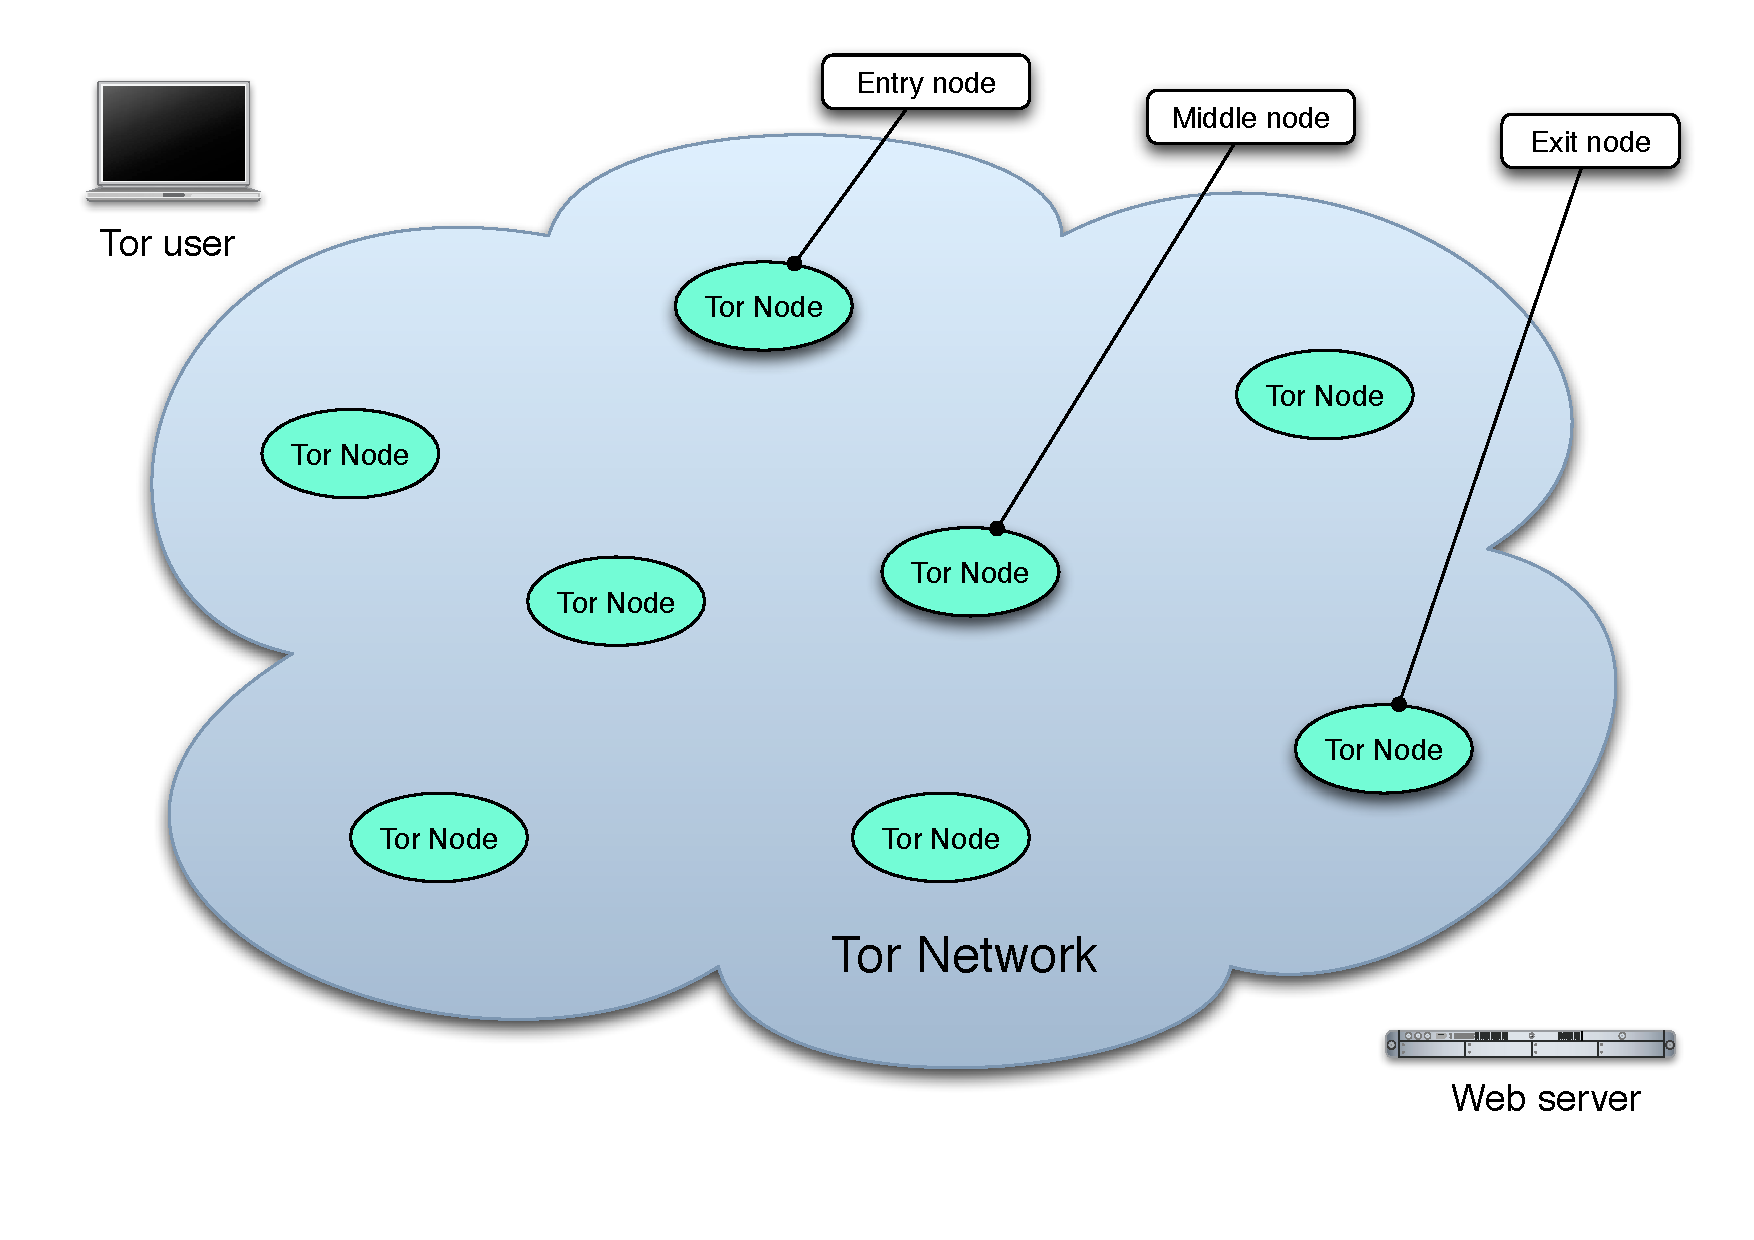
\includegraphics[keepaspectratio,width=\textwidth, height=.8\textheight]{images/tor-safe-selection}
\end{center}
\end{frame}
%----------------------------------------------------------------------------------------
\begin{frame}
\frametitle{Comment fonctionne Tor ?}
\begin{center}
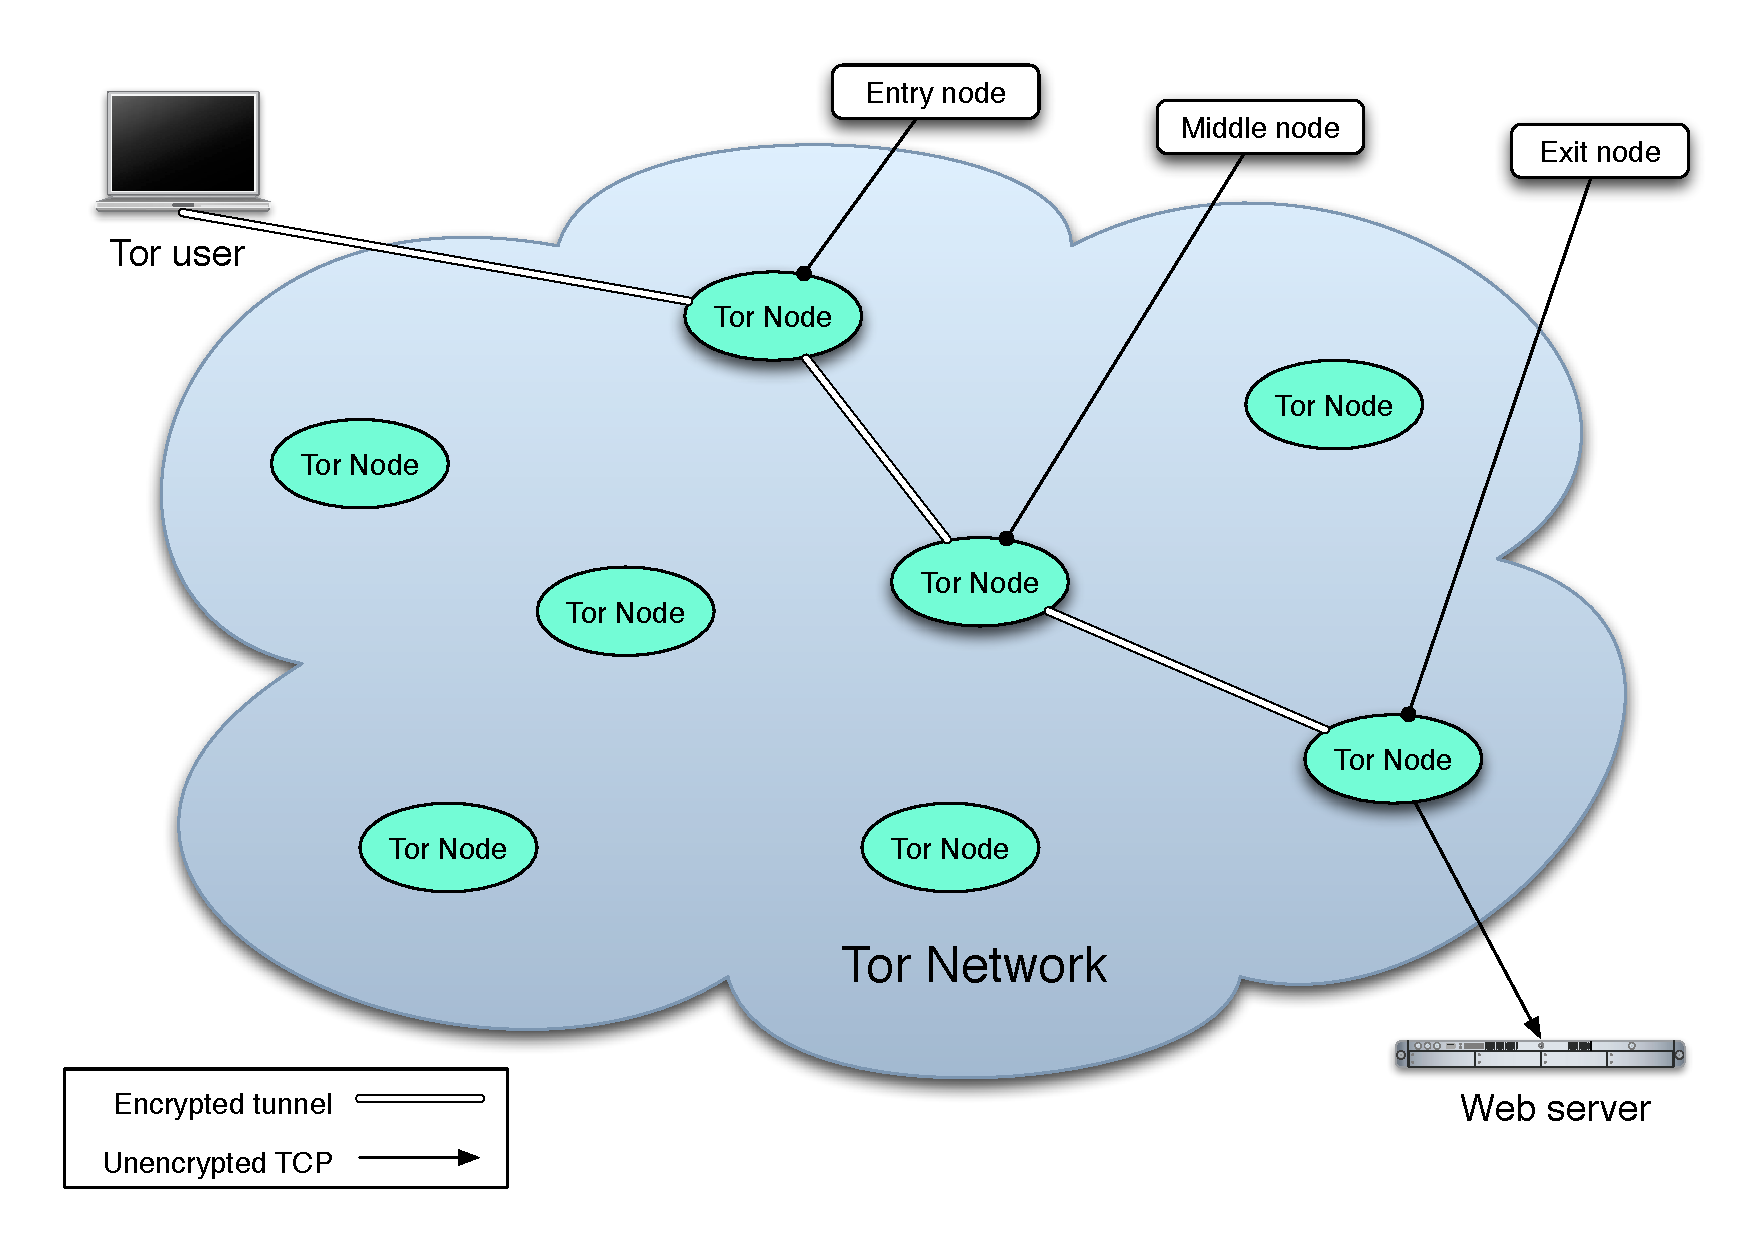
\includegraphics[keepaspectratio,width=\textwidth, height=.8\textheight]{images/tor-safe-path}
\end{center}
\end{frame}
%----------------------------------------------------------------------------------------
\begin{frame}
\frametitle{Comment fonctionne Tor ?}
\begin{center}
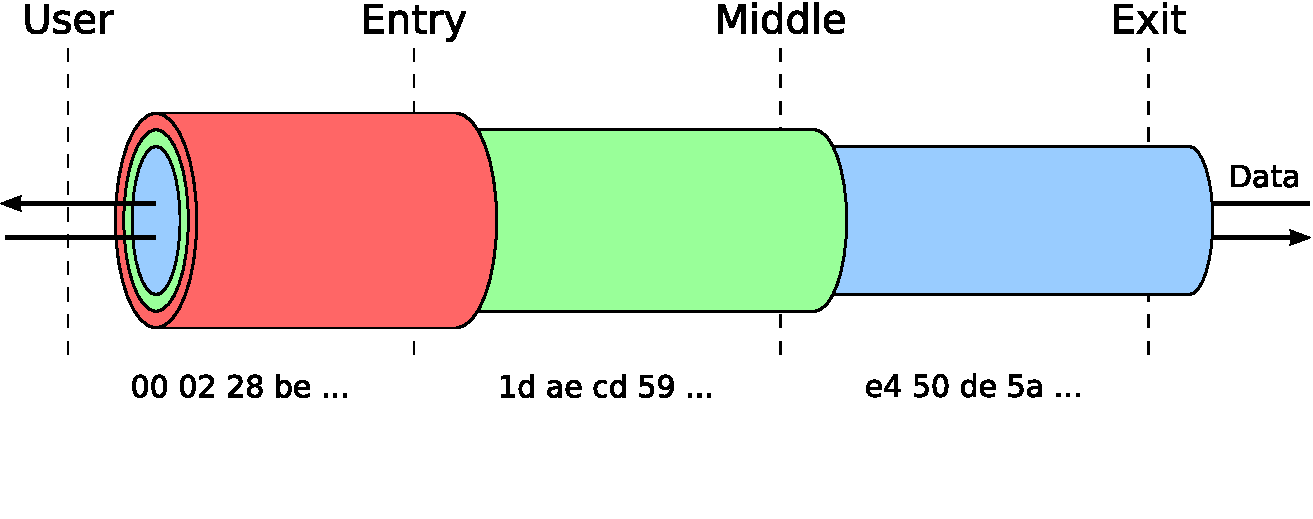
\includegraphics[keepaspectratio,width=\textwidth, height=.8\textheight]{images/tor-keys1}
\end{center}
\end{frame}
%----------------------------------------------------------------------------------------
\begin{frame}
\frametitle{Comment fonctionne Tor ?}
Ce tunnels se fait « en oignon » avec des couches de chiffrement empilées. Il y a une première
clé de chiffrement vers le nœud d'entrée, une second clé vers le nœud du milieu et
une dernière pour le nœud de sortie.
\\
Il faut noter que Tor ne s'occupe pas de chiffrer après le nœud de sortie. Comme n'importe
qui peut mettre en place un nœud de sortie, c'est une bonne idée de chiffrer sa communication
en plus (par exemple en se connectant aux sites web que l'on visite en HTTPS).
\\
Après, se déroule tout un processus pour établir un tunnel chiffré jusqu'au
nœud de sortie.
\end{frame}
%----------------------------------------------------------------------------------------
\begin{frame}
\begin{center}
\Huge{Tor hidden service \\ les services cachés de TOR}
\\~\\ 
\includegraphics[scale=0.4]{./images/logo_tor.jpg}
\end{center}
\end{frame}
%----------------------------------------------------------------------------------------
\begin{frame}
\frametitle{Tor hidden service - les services cachés de TOR}
Tor permet aux clients et aux relais d’offrir des services cachés.Il est possible d'offrir un serveur web, un serveur SSH, etc, sans révéler son adresse IP aux utilisateurs.
\begin{itemize}
\item Tous ces sites ne sont accessibles que via le réseau Tor.
\item Ils portent une adresse qui se termine par .onion.
\item Des wikis et moteurs de recherches référencient ces services.
\item Facebook, Wikipeida, des blogs...
\end{itemize}
\end{frame}
%----------------------------------------------------------------------------------------
\begin{frame}
\begin{center}
\Huge{Comment utiliser Tor ? }
\\~\\ 
\includegraphics[scale=0.4]{./images/logo_tor.jpg}
\end{center}
\end{frame}
%----------------------------------------------------------------------------------------
\begin{frame}
\frametitle{Utiliser Tor - Le Tor Browser}
Le Tor Browser est une version Extended Support de Firefox, auxquelles sont ajoutée les extensions préconfigurées permettant qu’au lancement du navigateur, celui-ci se connecte à Tor. 
\\$\Rightarrow$ Ainsi, toute la navigation qui se fait via ce navigateur est faite au travers du réseau Tor. 
\\$\Rightarrow$ Toutes les versions (dans différentes langues, différents OS) sont disponibles sur le site du projet : 
\\ \url{https://www.torproject.org/}
\end{frame}
%----------------------------------------------------------------------------------------
\begin{frame}
\begin{center}
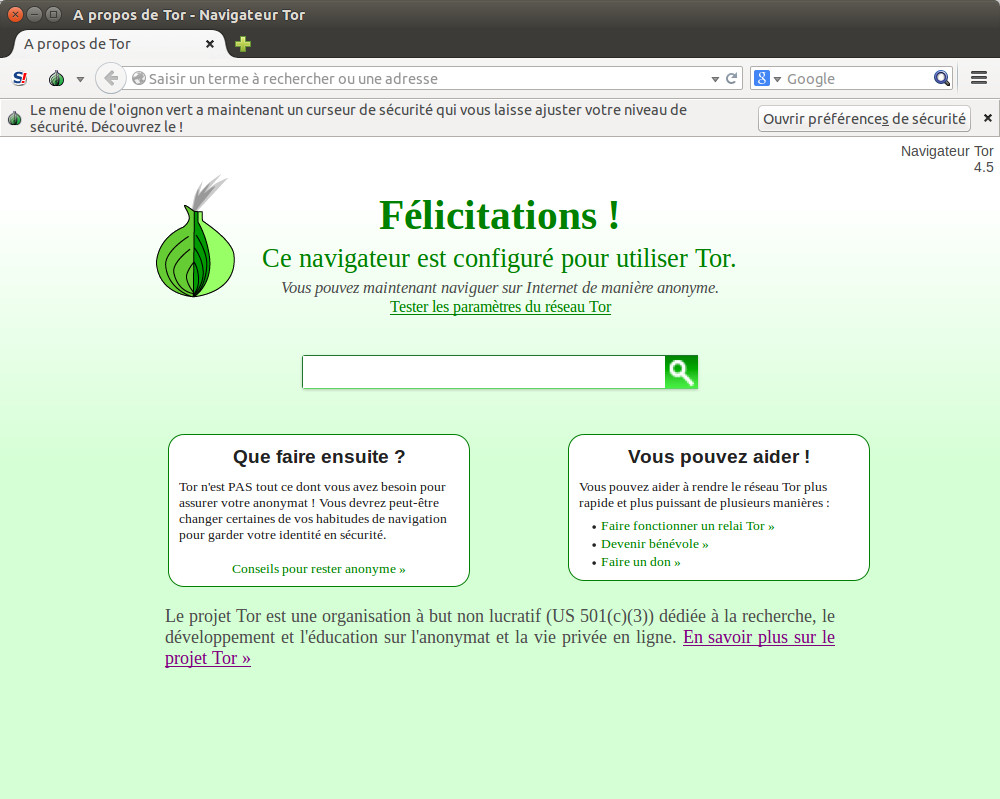
\includegraphics[scale=0.3]{./images/tor_browser03.jpg}
\end{center}
\end{frame}
%----------------------------------------------------------------------------------------
\begin{frame}
\frametitle{Tor Browser Launcher}
Pour avoir un Tor Browser toujours à jour, on peut installer le Tor Browser Launcher.
\begin{center}
\url{https://github.com/micahflee/torbrowser-launcher}
\\ 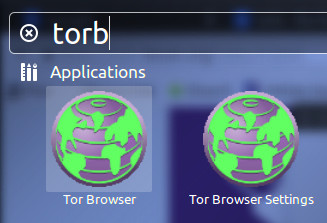
\includegraphics[scale=0.3]{./images/tor_browser01.jpg}
\\ 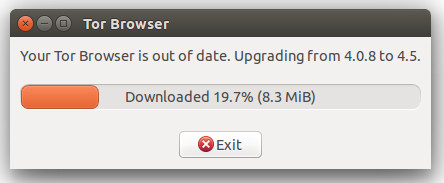
\includegraphics[scale=0.3]{./images/tor_browser02.jpg}
\end{center}
\end{frame}
%----------------------------------------------------------------------------------------
\begin{frame}
\frametitle{Tor Browser Launcher}
Il gère : 
\begin{itemize}
\item le téléchargement de la version la plus récente de TBB, dans votre langue et pour votre architecture
\item la mise à jour automatique (tout en conservant vos signets et préférences) manuel
\item la vérification de la signature GnuPG du TBB (pour être sûr de l’intégrité des fichiers)
\item ajoute un lanceur d’application "Tor Browser" dans le menu de votre environnement de bureau.
\end{itemize}
\end{frame}
%----------------------------------------------------------------------------------------
\begin{frame}
\begin{center}

\includegraphics[scale=0.3]{./images/tails_logo.jpg}
\\~\\
\url{https://tails.boom.org}
\end{center}
\end{frame}
%----------------------------------------------------------------------------------------
\begin{frame}
\frametitle{Utiliser Tor - Tails}
Tails est un système d'exploitation complet basé sur Linux et Debian, en live.
\begin{center}
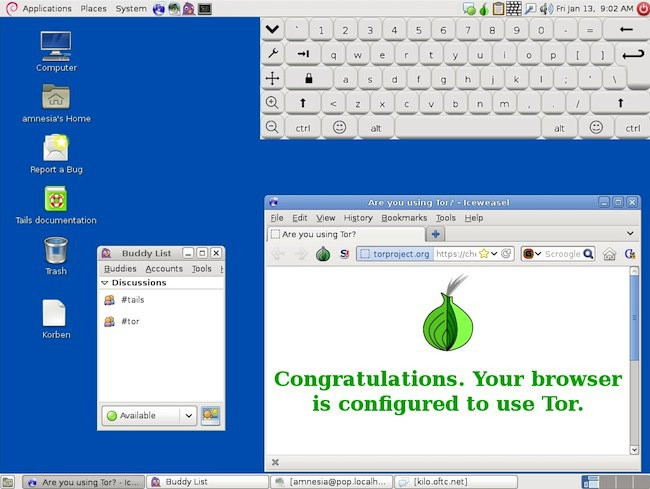
\includegraphics[scale=0.3]{./images/tails.jpg}
\\~\\
\url{https://tails.boom.org}
\end{center}
\end{frame}
%----------------------------------------------------------------------------------------
\begin{frame}
\begin{center}
\Huge{Vous voulez que Tor \\ marche vraiment ?}
\\~\\ 
\includegraphics[scale=0.4]{./images/logo_tor.jpg}
\end{center}
\end{frame}
%----------------------------------------------------------------------------------------
\begin{frame}
\frametitle{Vous voulez que Tor marche vraiment ?}
Vous devrez changer quelques-unes de vos habitudes, et certaines choses ne marcheront pas exactement comme vous le voudrez.
\begin{itemize}
\item Ne faîte pas de Torrent via Tor
\item N'activez pas et n'installez pas de plugins dans le navigateur
\item Utiliser la version HTTPS des sites webs
\item Ne consultez pas/n'ouvrez pas de documents téléchargé pendant que vous êtes connecté via Tor
\end{itemize}
\end{frame}
%----------------------------------------------------------------------------------------
\begin{frame}
\begin{center}
\Huge{Soutenir le projet Tor}
\\~\\ 
\includegraphics[scale=0.4]{./images/logo_tor.jpg}
\end{center}
\end{frame}
%---------------------------------------------------------------------------------------
\begin{frame}
\frametitle{Soutenir le projet Tor}
Il existe l'association NosOignons.net, qui propose des nœuds de sortie Tor financés par la communauté.
\url{https://nos-oignons.net}
\begin{itemize}
\item En parler
\item Faire un don à NosOignons
\item Devenir membre de la communauté
\item Faire des tutoriaux, de la traduction, contibuez au code...
\end{itemize}
\end{frame}
%------------------------------------------------
\begin{frame}
\frametitle{Les cafés vie privée}
\begin{center}

\includegraphics[scale=0.4]{./images/LogoCafeViePrivee.jpg}
\\ \url{https://café-vie-privée.fr/}
\\ @chiffrofete \#cafevieprivee
\end{center}
\end{frame}
%----------------------------------------------------------------------------------------
\begin{frame}
\begin{center}
\Huge{Questions et discussion}
\end{center}
\end{frame}
%----------------------------------------------------------------------------------------
\end{document}
